\documentclass{beamer}

% Theme and color scheme
\usetheme{Madrid}
\usecolortheme{default}

% Font package (optional)
\usepackage{helvet}

% Additional packages
\usepackage{graphicx}
\usepackage{booktabs}
\usepackage{amsmath}

\usepackage{xcolor} % Required for defining colors

% Define custom colors
\definecolor{ETH_Blue}{RGB}{33, 92, 175} 
\definecolor{ETH_Brown}{RGB}{142, 103, 19} 
\definecolor{ETH_Green}{RGB}{98, 115, 19} % Green
\definecolor{ETH_Red}{RGB}{183, 53, 45} % Red
\definecolor{ETH_Grey}{RGB}{111, 111, 111} % Grey
\definecolor{ETH_Background}{RGB}{255, 255, 255} % White
\definecolor{ETH_Text}{RGB}{0, 0, 0} % Black


\setbeamercolor{frametitle}{bg=ETH_Blue, fg=ETH_Background}
\setbeamercolor{title}{bg=ETH_Blue, fg=ETH_Background}
\setbeamercolor{section in toc}{fg=ETH_Blue}
\setbeamercolor{subsection in toc}{fg=ETH_Text}
\setbeamercolor{item}{fg=ETH_Blue}
\setbeamercolor{itemize item}{fg=ETH_Blue}
\setbeamercolor{enumerate item}{fg=ETH_Blue}
%\setbeamercolor{block title}{bg=ETH_Green, fg=ETH_Background}
%\setbeamercolor{block body}{bg=ETH_Background, fg=ETH_Text}
\setbeamercolor{alerted text}{fg=ETH_Red}
\setbeamercolor{normal text}{fg=ETH_Text}
\setbeamercolor{footline}{bg=ETH_Grey, fg=ETH_Background}

\setbeamertemplate{footline}[page number]
\setbeamertemplate{navigation symbols}{}

% Title, author, and date
\title{Planar Graphs Have Bounded Queue-Number}
\author{Shengzhe Wang}
\institute{ETH Zürich}
\date{\today}

\begin{document}
	
	% Title slide
	\begin{frame}
		\titlepage
	\end{frame}
	
	
	
	% Section 1
	\section{Introduction to Queue-Number}
	\subsection{Queue Layout}
	\begin{frame}
		\frametitle{Queue Layout}
		
		
		\begin{center}
			\onslide<1-2>{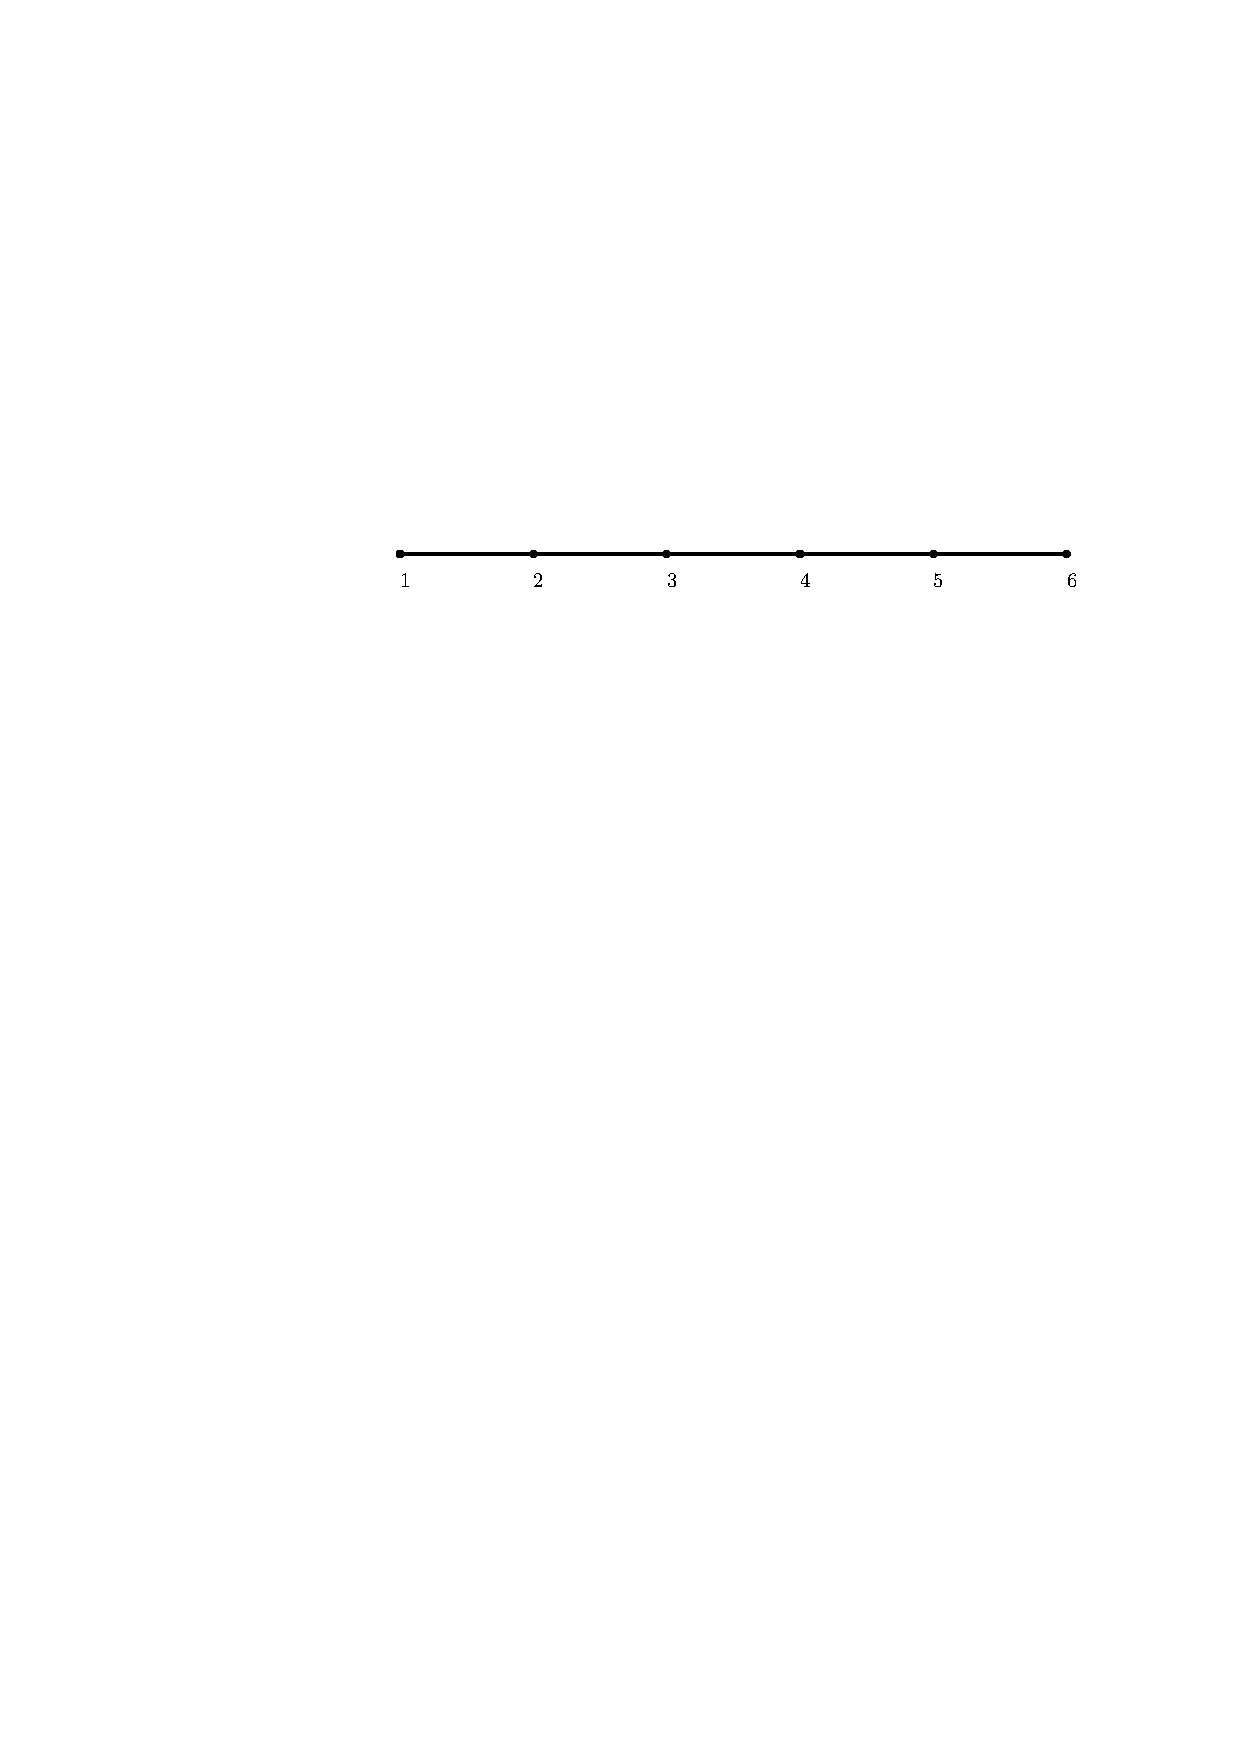
\includegraphics[width=0.8\textwidth]{pics/1_6_queue.pdf}} \\
			\vspace{1.5cm}
			\onslide<2->{
				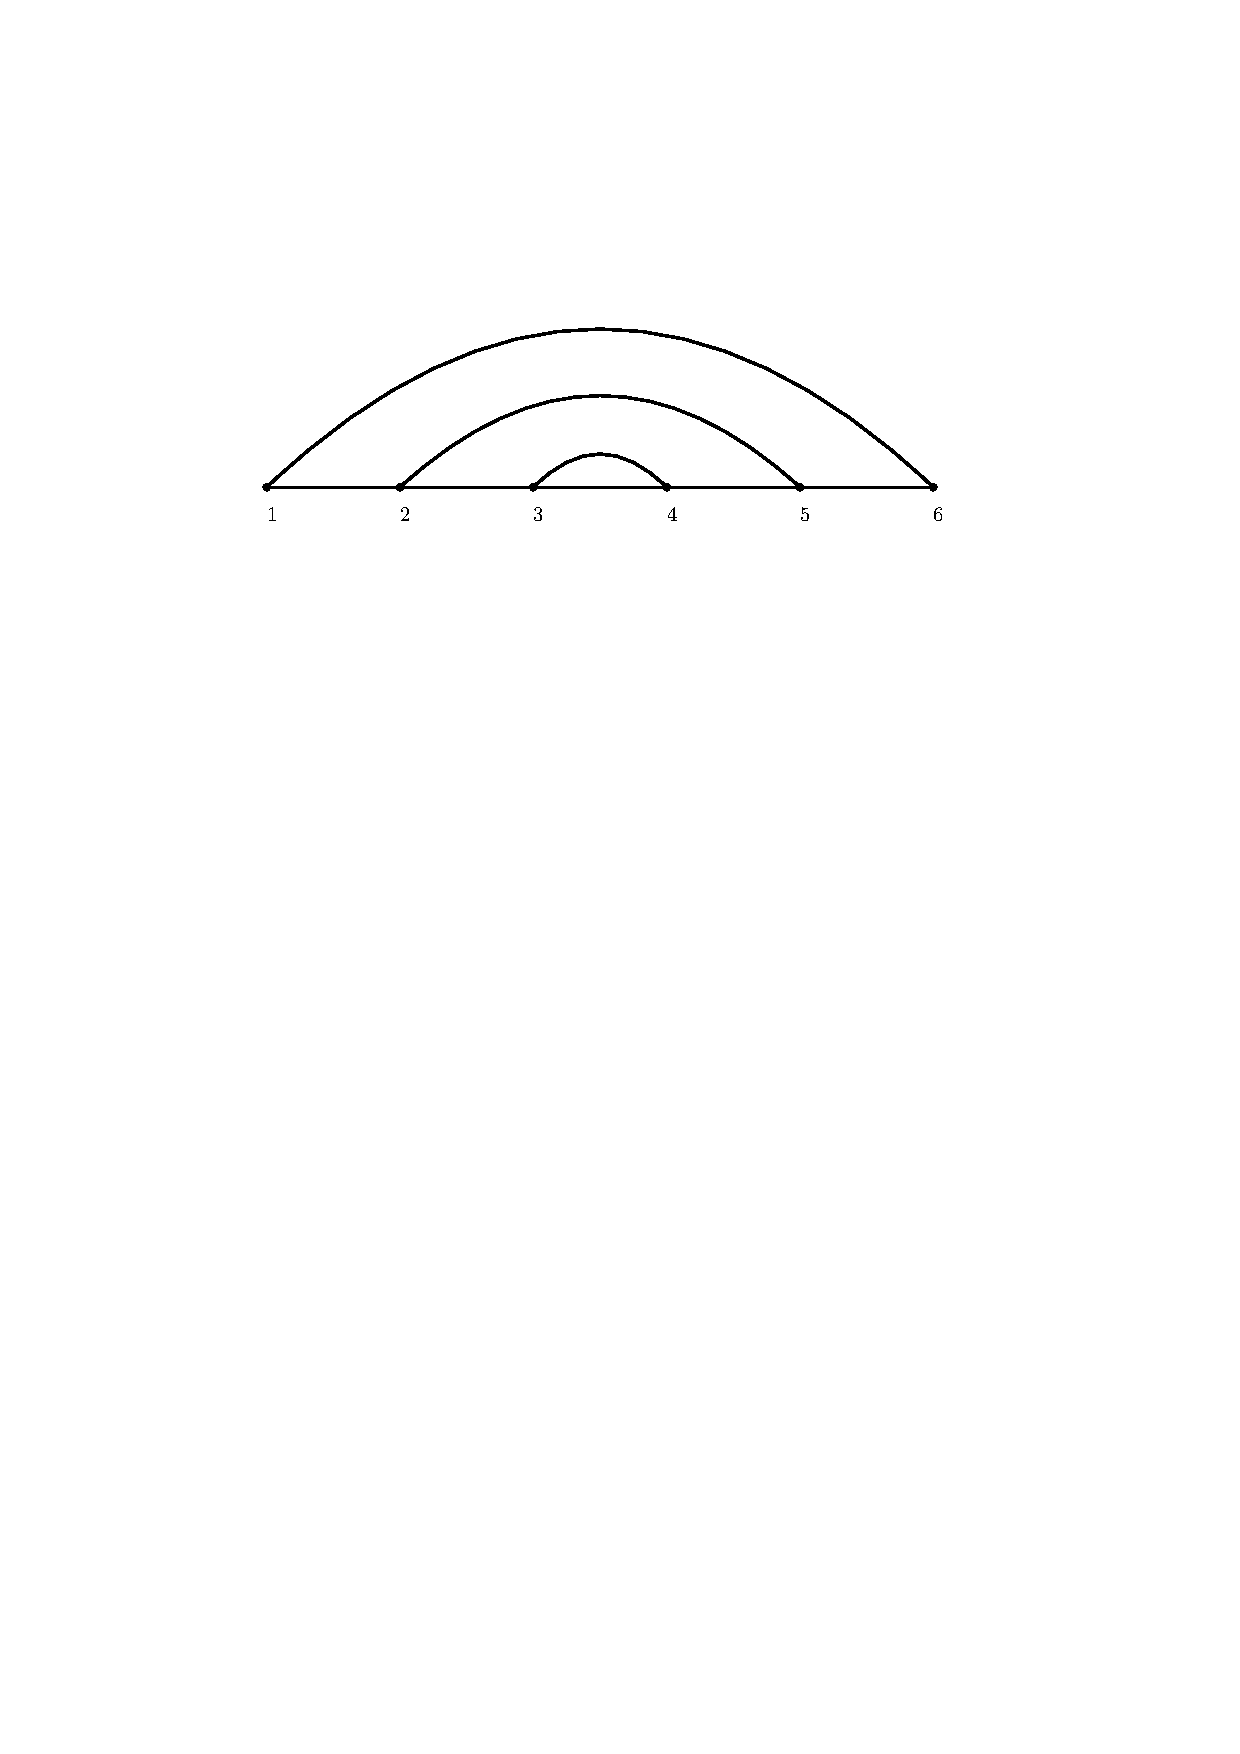
\includegraphics[width=0.8\textwidth]{pics/1_6_invalid_queue.pdf}}\\
			\vspace{0.25cm}
			\onslide<3->{Not Valid Queue-Layout}
		\end{center}
		
	\end{frame}
	
	\begin{frame}
		\frametitle{Queue Layout}
		\begin{center}
			\includegraphics<1>[width=0.75\textwidth]{pics/colored_queue.pdf}
			\includegraphics<2>[width=0.75\textheight]{pics/colored_queue_1.pdf}
			\includegraphics<3>[width=0.75\textheight]{pics/colored_queue_2.pdf}
			\includegraphics<4>[width=0.75\textheight]{pics/colored_queue_3.pdf}
		\end{center}
	\end{frame}
	
	\begin{frame}
		\frametitle{Queue Layout}
		\begin{block}{Definition: Queue}
			Let $G = (V,E)$, consider a linear odering $\preceq$ of $V$, a queue of $G$ is a set of edges $E^\prime \subseteq E$ such that any disjoint edges $vw,xy \in E^\prime$, w.l.o.g, $v \prec w, x \prec y$ and $v \prec x$, we have $w \prec y$.
		\end{block}
		\begin{center}
			%\vspace{0.5cm}
			\vfill
			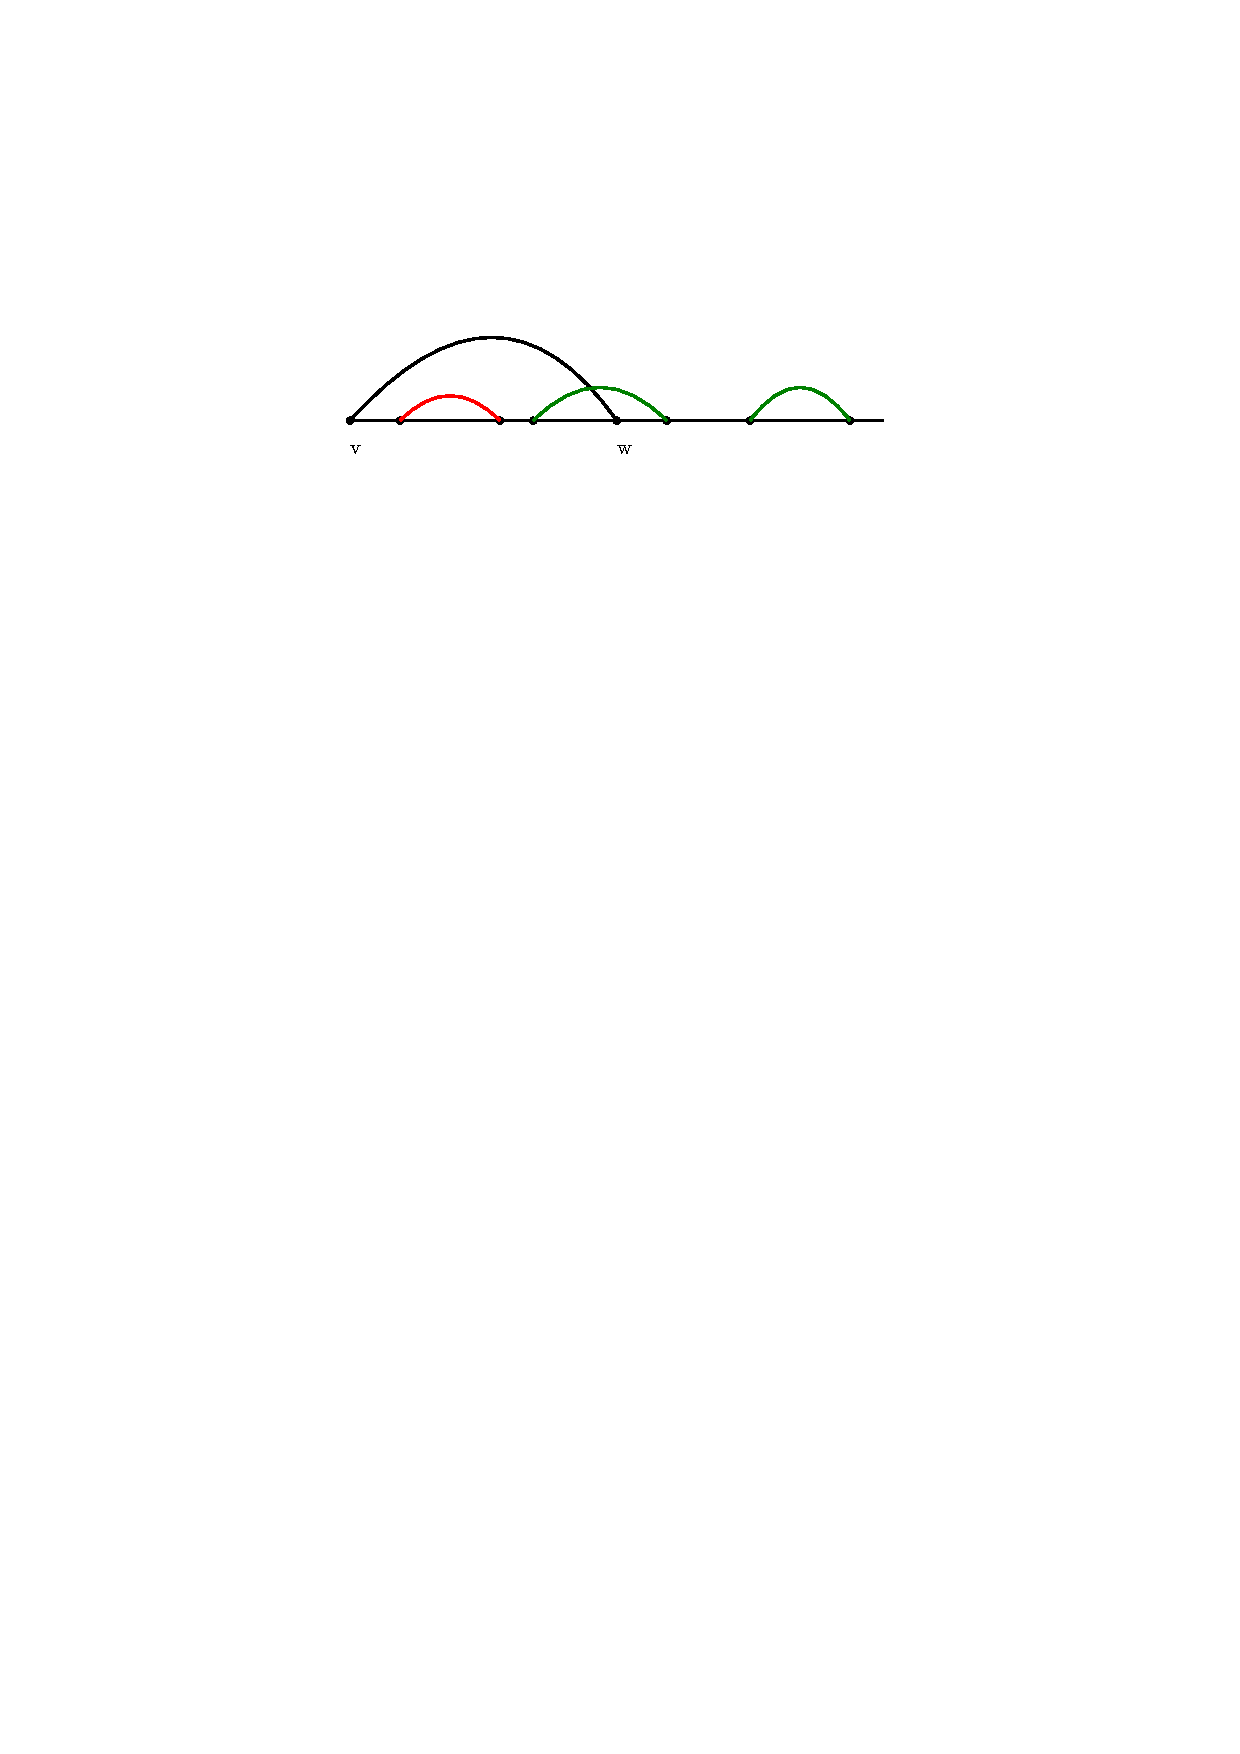
\includegraphics[width=0.75\textwidth]{pics/vwxy.pdf}
		\end{center}
	\end{frame}
	
	\subsection{Queue-Number}
	\begin{frame}
		\frametitle{Queue-Number}
		\onslide<1->
		{
			\begin{block}{Definition: K-Queue Layout}
				Let $G = (V,E)$, consider a linear odering $\preceq$ of $V$, for an integer $k \ge 0$ a $k$-queue layout of $G$ is a partition of $E$ into $E_1,E_2,...,E_k$ such that each $E_i$ is a queue of $G$.
			\end{block}
		}\pause
		
		\onslide<2->
		{
			\begin{block}{Definition: Queue-Number}
				The queue-number of $G$, denoted by qn$(G)$, is the minimum integer $k$ such that $G$ has a $k$-queue layout.
			\end{block}
		}
	\end{frame}
	
	\begin{frame}
		\frametitle{Queue-Number: Tree}
		\begin{center}
			What is the queue-number of tree?
			\vfill
			\includegraphics<1>[width=0.6\textwidth]{pics/qn_tree.pdf}
			\includegraphics<2>[width=0.6\textwidth]{pics/qn_tree_labeled.pdf}
			\includegraphics<3>[width=0.5\textwidth]{pics/qn_tree_labeled.pdf}
			\vfill
			\includegraphics<3>[width=0.7\textwidth]{pics/qn_tree_layered.pdf}
		\end{center}
	\end{frame}
	
	\begin{frame}
		\frametitle{Queue Number: Cycle}
		\begin{center}
			\onslide<1->{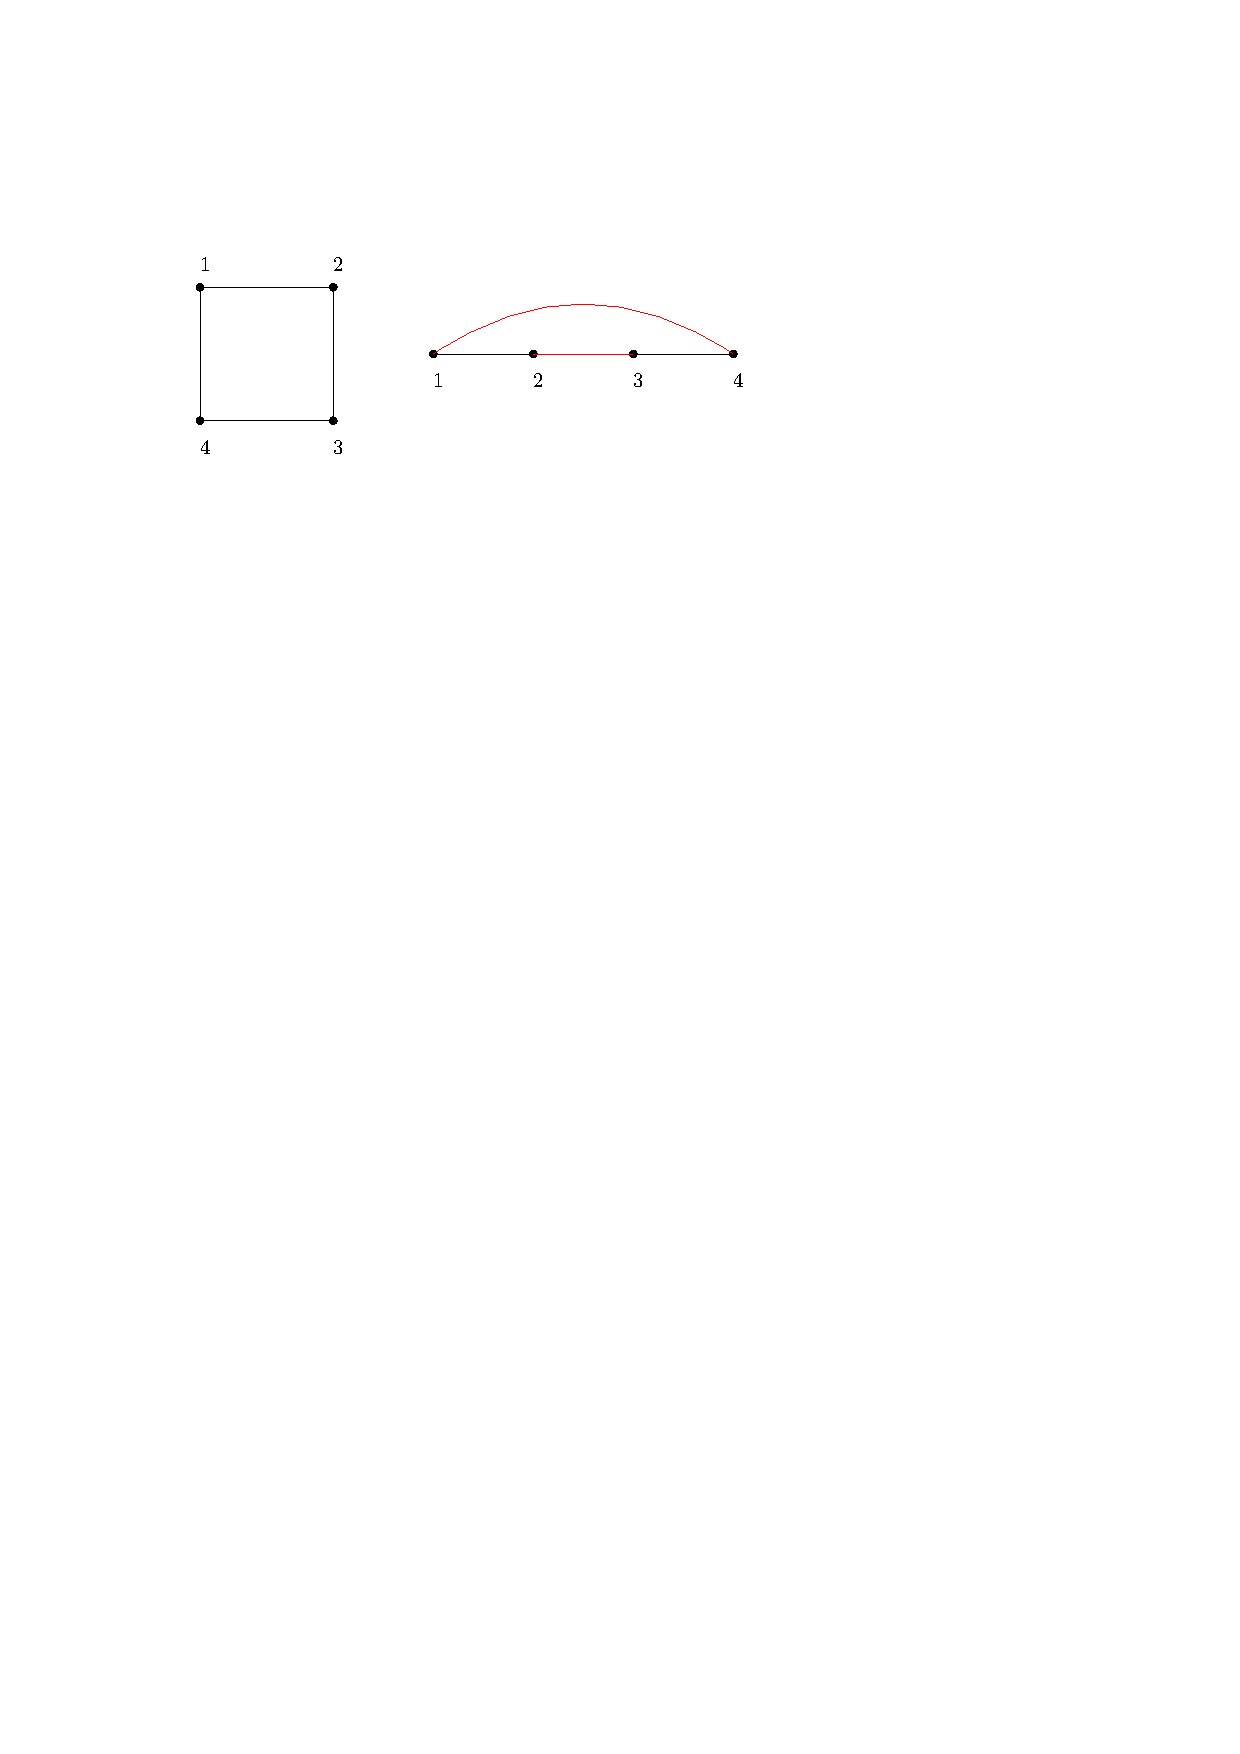
\includegraphics[width=0.5\textwidth]{pics/qn_cycle_label1.pdf}} \\
			\vfill
			\onslide<2->{
				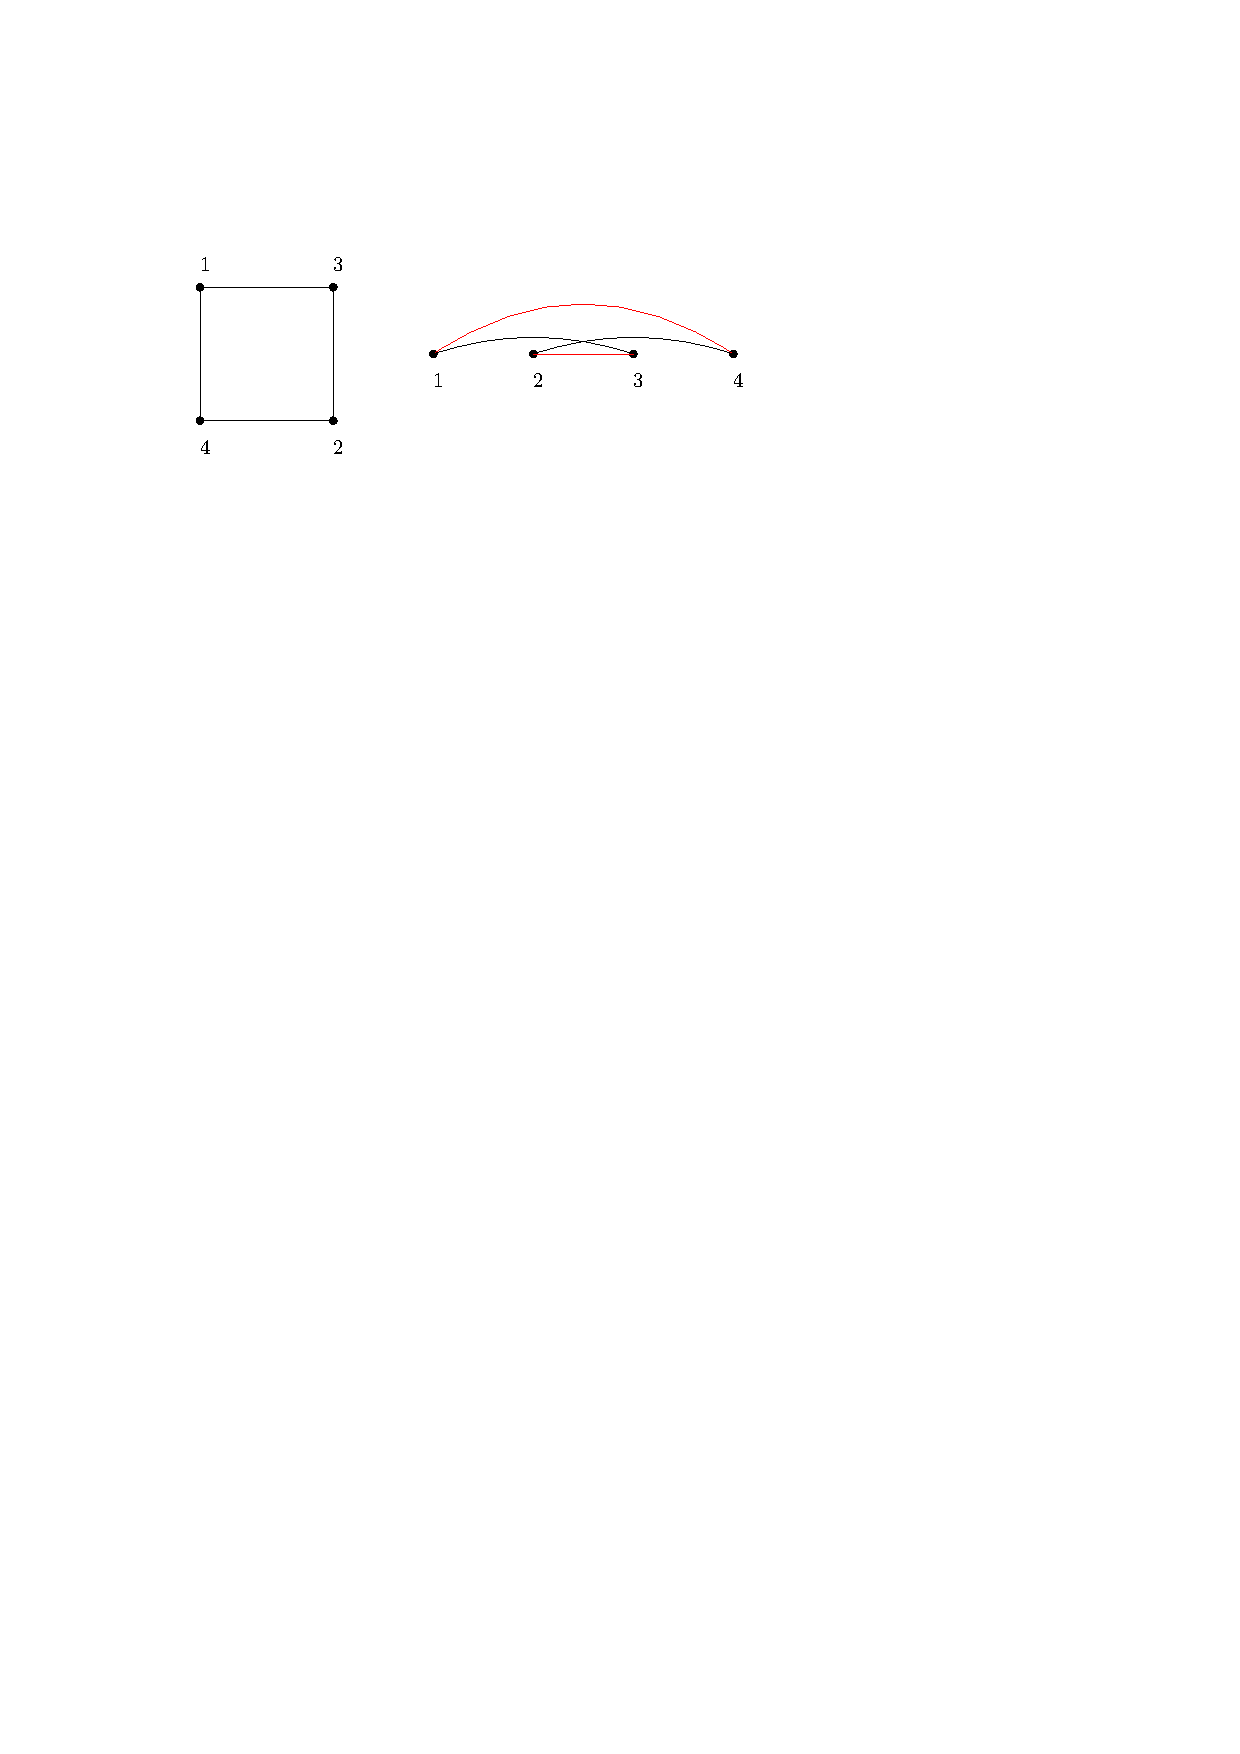
\includegraphics[width=0.5\textwidth]{pics/qn_cycle_label2.pdf}}\\
			\vfill
			\onslide<3->{
				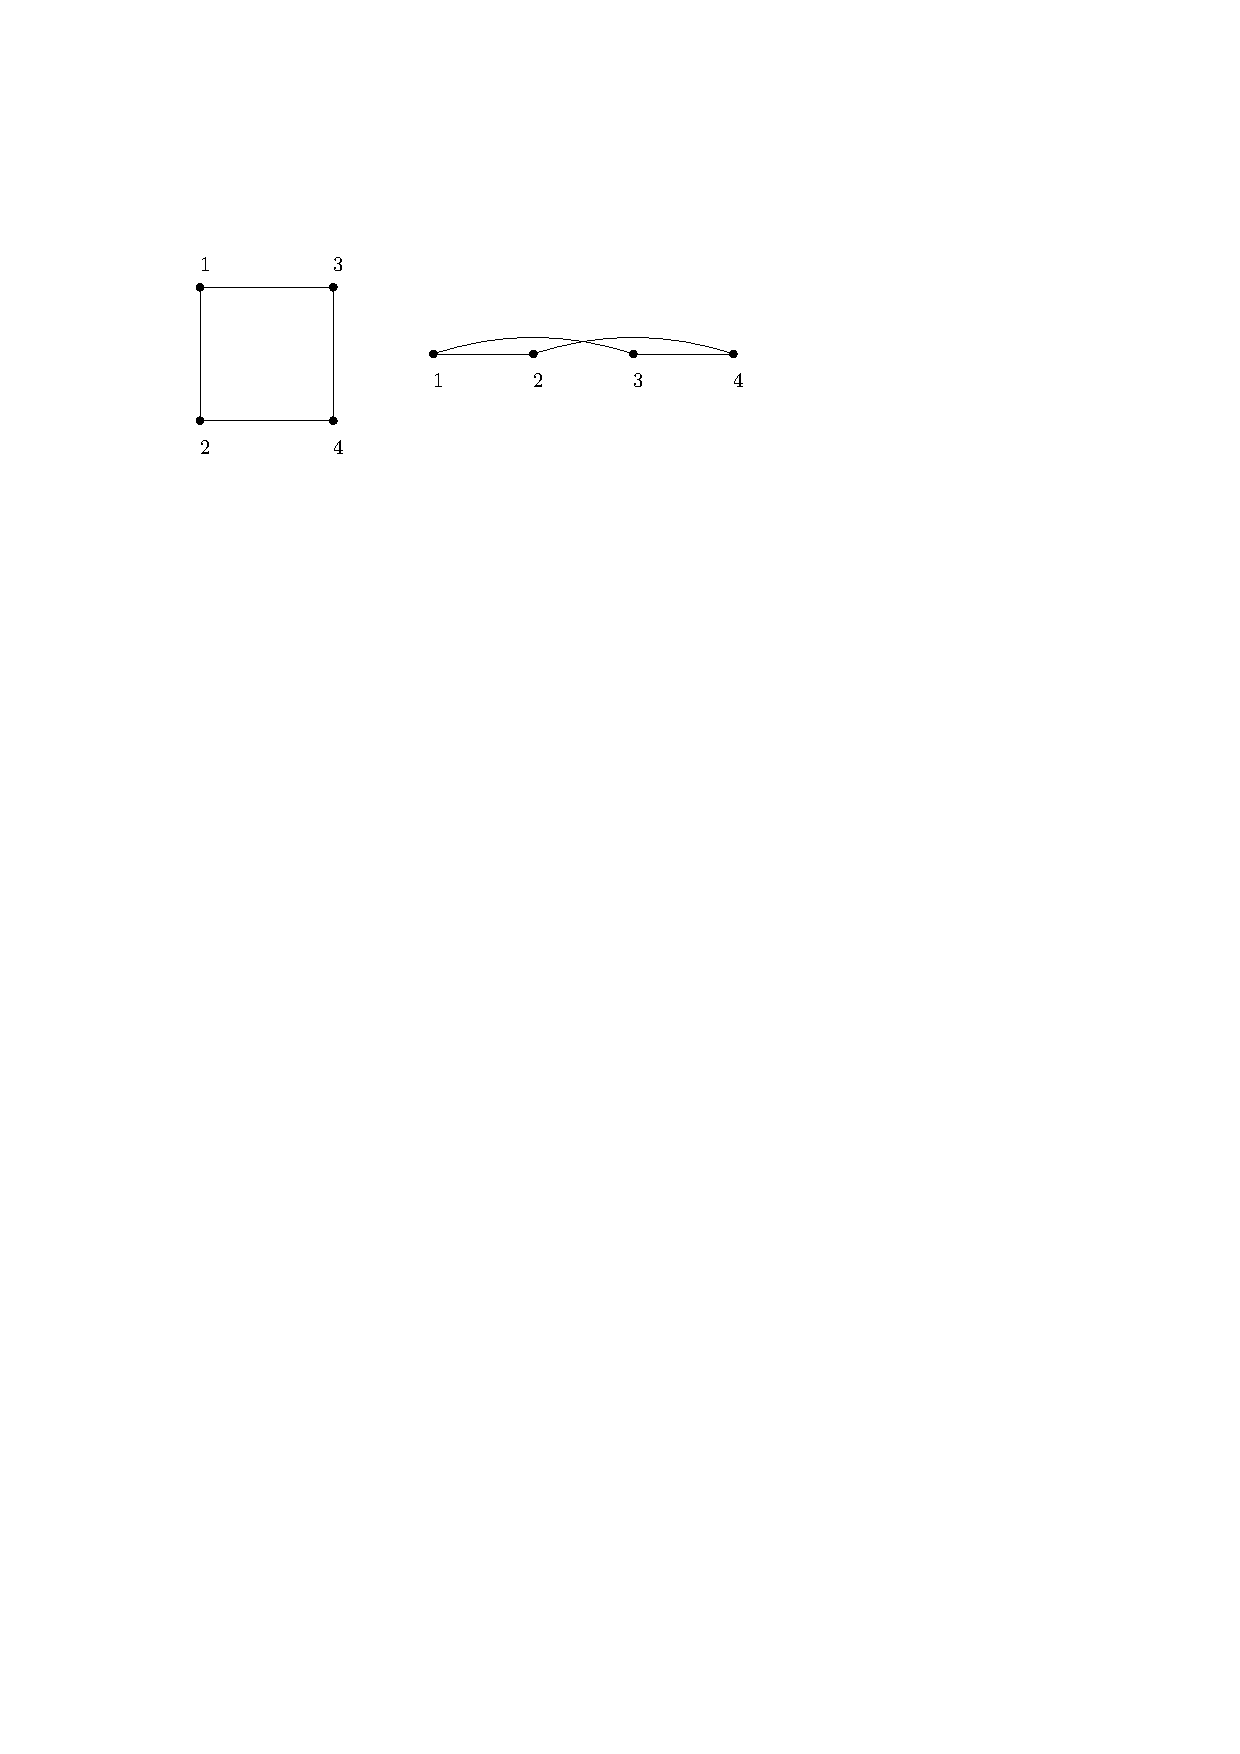
\includegraphics[width=0.5\textwidth]{pics/qn_cycle_label3.pdf}}\\
		\end{center}
	\end{frame}
	
	\section{Introduction to Treewidth}
	\subsection{Treewidth}
	\begin{frame}
		\frametitle{Treewidth}
		\onslide<1->{Do we have some tools to help bound the queue-number?}
		\vspace{1cm}
		\onslide<2->
		{
			\begin{theorem}[Veit,2017]
				Every graph with treewidth $k$ has queue-number at most $2^k-1$.
			\end{theorem}
		}
	\end{frame}

	\begin{frame}
		\frametitle{Tree-decomposition}
		\begin{block}{Definition: Tree-decomposition}
			A tree-decomposition of a graph $G$ is a pair $(B,T)$. $T$ is a tree and $B = \{B_x | x \in V(T)\}$ where each $B_x$ is a subset of $V(G)$ for every vertex $x$ in $V(T)$ such that
			\begin{itemize}
				\item $\forall \{v,w\} \in E(G)$, there exists $x \in V(T)$ with $v,w \in B_x$
				\item $\forall v \in V(G)$, the set $\{x| x \in V(T) \wedge v \in B_x\}$ induces a non -empty connected subtree of $T$.
			\end{itemize}
		\end{block}
		\begin{center}
			\includegraphics<1>[width=0.15\textwidth]{pics/treewd_G.pdf}
			\includegraphics<2>[width=0.4\textwidth]{pics/treewd_T.pdf}
			\includegraphics<3>[width=0.4\textwidth]{pics/treewd_TB.pdf}
			\includegraphics<4>[width=0.4\textwidth]{pics/treewd_TB_simp.pdf}
			\includegraphics<5>[width=0.4\textwidth]{pics/treewd_TB_bad2.pdf}
			\includegraphics<6>[width=0.4\textwidth]{pics/treewd_TB_bad1.pdf}
			\includegraphics<7>[width=0.4\textwidth]{pics/treewd_TB_bad3.pdf}
		\end{center}
	\end{frame}

	\begin{frame}
		\frametitle{Treewidth}
		\onslide<1->
		{
			\begin{block}{Definition: Tree-decomposition}
				A tree-decomposition of a graph $G$ is a pair $(B,T)$. $T$ is a tree and $B = \{B_x | x \in V(T)\}$ where each $B_x$ is a subset of $V(G)$ for every vertex $x$ in $V(T)$ such that
				\begin{itemize}
					\item $\forall \{v,w\} \in E(G)$, there exists $x \in V(T)$ with $v,w \in B_x$
					\item $\forall v \in V(G)$, the set $\{x| x \in V(T) \wedge v \in B_x\}$ induces a non -empty connected subtree of $T$.
				\end{itemize}
			\end{block}
			\begin{block}{Definition: Width of Tree-decomposition}
				The width of a tree-decomposition of $G$ is $\max_{x \in V(T)} |B_x| - 1$
			\end{block}
		}
		\onslide<2>
		{
			\begin{block}{Definition: Treewidth}
				The treewidth of a graph $G$ is the minimum width of all tree-decomposition of $G$. 
			\end{block}
		}
		
	\end{frame}

	\begin{frame}
		\frametitle{Treewidth: Tree}
		\begin{center}
			\includegraphics<1>[width=0.4\textwidth]{pics/treewd_tree_base.pdf}
			\includegraphics<2->[width=0.8\textwidth]{pics/treewd_tree.pdf}
			\vfill
			\onslide<3>{Tree has treewidth 1}
		\end{center}
	\end{frame}

	\begin{frame}
		\frametitle{Treewidth: Planar graph}
		\onslide<1->
		{
			\begin{theorem}[Veit,2017]
				Every graph with treewidth $k$ has queue-number at most $2^k-1$.
			\end{theorem}
			\vfill
			If planar graph has bounded treewidth, then planar graph has bounded queue-number.
		}
	
		\onslide<2->
		{
			\vfill
			\begin{theorem}
				Planar graph on $n$ vertices has treewidth $O(\sqrt{n})$ and the bound is tight.
			\end{theorem}
		}
		\onslide<3>
		{
			\begin{center}
				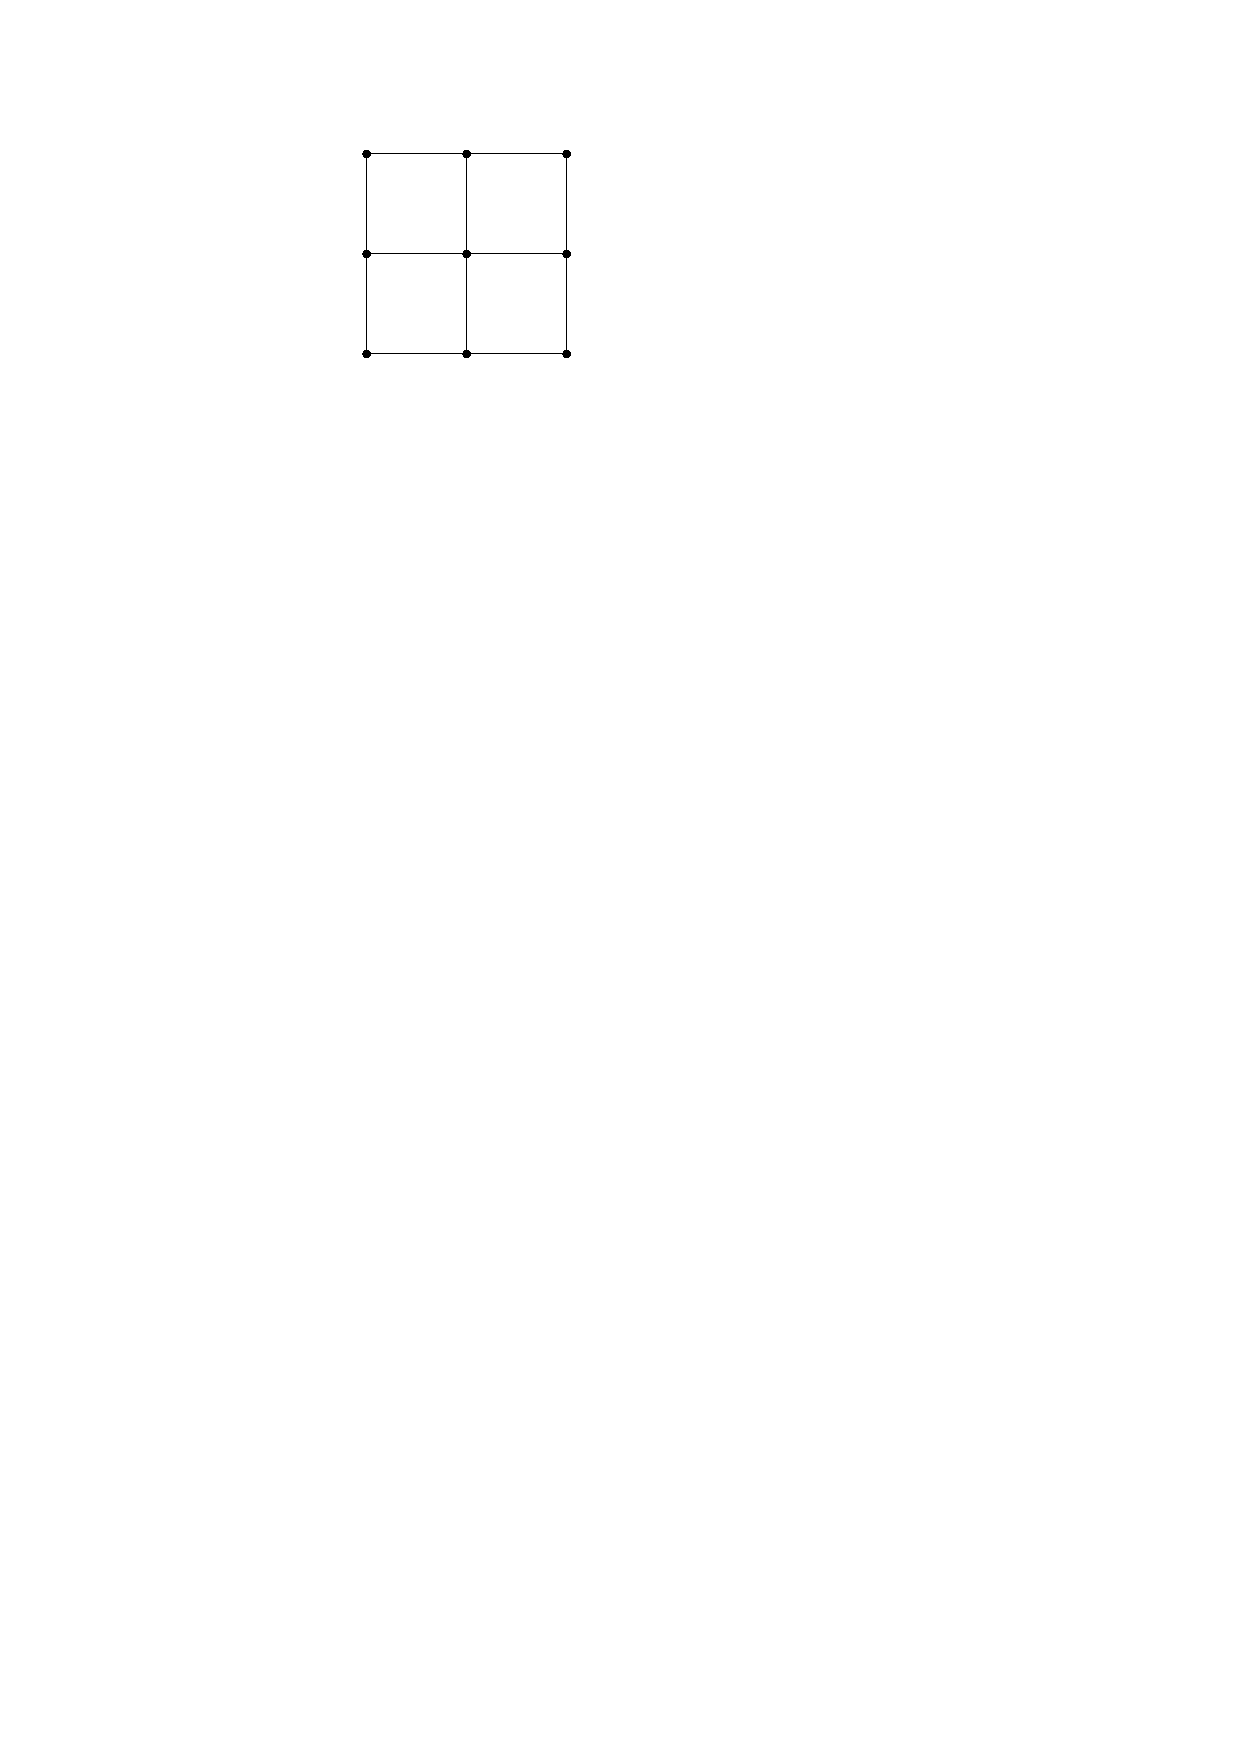
\includegraphics[width=0.2\textwidth]{pics/treewd_grid.pdf}
			\end{center}
		}
		
	\end{frame}

	\section{Introduction to Partitions}
	\subsection{Partitions}
	\begin{frame}
		\frametitle{Partitions}
		\onslide<1->{Maybe we need more structures}
		\vfill
		\onslide<2->
		{
			\begin{theorem}[Vida et al.,2020]
				For a graph $G$, if $G$ has an $H$-partition of layered width $l$ and $H$ has treewidth $k$, then 
				
				$$\text{qn}(G) \le 3l(2^k-1) + \lfloor \frac{3}{2} l \rfloor$$
			\end{theorem}
		}
	\end{frame}

	\begin{frame}
		\frametitle{Partitions}
		\onslide<1->
		{
			\begin{block}{Definition: Partition and Quotient}
				A partition of $G$ is a set $\mathcal{P} = \{P_1,...,P_n\}$ of non-empty subsets of $V(G)$ and each vertex of $G$ is in exactly one element (part) of $\mathcal{P}$.
				
				The quotient of $\mathcal{P}$ is a graph, denoted by $G/\mathcal{P}$, with each vertex $v_i$ corresponds $P_i$. For any two vertices $v_i,v_j$ in $G/\mathcal{P}$, they are connected if and only if some vertex in $P_i$ is connected to some vertex in $P_j$ in graph $G$.
			\end{block}
		}
		\onslide<5->
		{
			\begin{block}{Definition: $H$-partition}
				A $H$-partition of a graph $G$ is a pair $(A,H)$. $A = \{A_x | x \in V(H)\}$ is a partition of $V(G)$ and $H$ is a graph isomorphic to the quotient $G/A$.
			\end{block}
		}
	\vfill
		\begin{center}
			\includegraphics<2>[width=0.3\textwidth]{pics/partition_G.pdf}
			\includegraphics<3>[width=0.3\textwidth]{pics/partition_P.pdf}
			\includegraphics<4-5>[width=0.6\textwidth]{pics/partition_H.pdf}
			\includegraphics<6>[width=0.6\textwidth]{pics/partition_bad1.pdf}
			\includegraphics<7>[width=0.6\textwidth]{pics/partition_bad2.pdf}
		\end{center}
	\end{frame}

	\subsection{Layering}
	\begin{frame}
		\frametitle{Layering}
		\begin{center}
			\includegraphics<1>[width=0.7\textwidth]{pics/layering.pdf}
			\includegraphics<2>[width=0.9\textwidth]{pics/path_partition.pdf}
		\end{center}
	\end{frame}


	\subsection{Layered Width}
	\begin{frame}
		\frametitle{Layered width}
		\begin{block}{Definition: Layered width}
			The layered width of a partition $\mathcal{P}$ of a graph $G$ is the minimum integer $l$ such that there exists a path-partition (layering) of $G$, each element in $\mathcal{P}$ has at most $l$ vertices in each element of path-partition.
		\end{block}
		\vfill
		\begin{center}
			\includegraphics<2>[width=0.4\textwidth]{pics/layerwd_partition.pdf}
			\includegraphics<3>[width=0.4\textwidth]{pics/layerwd_layering_w3.pdf}
			\includegraphics<4>[width=0.4\textwidth]{pics/layerwd_layering_w1.pdf}
		\end{center}
	\end{frame}

	\subsection{Vertical Path}
	\begin{frame}
		\frametitle{Layered width: Tree}
		\begin{block}{Definition: Vertical Path}
			Let $T$ be a tree rooted at a vertex $r$, a non-empty path $(x_1,...,x_p)$ in $T$ is vertical if for some $d \ge 0$ and for all $1 \le i  \le p$ we have $\text{dist}_T(x_i,r) = d+i$.
		\end{block}
		\vfill
		\begin{center}
			\includegraphics<2>[width=0.25\textwidth]{pics/vp_tree.pdf}
			\includegraphics<3>[width=0.25\textwidth]{pics/vp_tree_p1.pdf}
			\includegraphics<4>[width=0.25\textwidth]{pics/vp_tree_p2.pdf}
			\includegraphics<5>[width=0.25\textwidth]{pics/vp_tree_p3.pdf}
			\includegraphics<6>[width=0.25\textwidth]{pics/vp_tree_partition.pdf}
			\includegraphics<7->[width=0.3\textwidth]{pics/vp_tree_partition_lw1.pdf}
		\end{center}
		\onslide<8>{A partition of the tree where each part is a vertical path has layered width 1.}
	\end{frame}

	\section{Planar Graph Decomposition}
	\begin{frame}
		\frametitle{Planar Graph Decomposition}
		\onslide<1->
		{
			\begin{theorem}[Vida et al.,2020]
				For a graph $G$, if $G$ has an $H$-partition of layered width $l$ and $H$ has treewidth $k$, then 
				
				$$\text{qn}(G) \le 3l(2^k-1) + \lfloor \frac{3}{2} l \rfloor$$
			\end{theorem}
		}
		\vfill
		\onslide<2->
		{
			\begin{theorem}[Vida et al.,2020]
				Every planar graph $G$ has a connected partition $\mathcal{P}$ with layered width 1 such that $H = G/\mathcal{P}$ has treewidth at most 8.
			\end{theorem}
		}
		\vfill
		\onslide<3->
		{
			\begin{theorem}[Vida et al.,2020]
				Every planar graph $G$ has queue-number at most 
				$$3(2^8-1) + \lfloor \frac{3}{2} \rfloor = 766$$ 
			\end{theorem}
		}
	\end{frame}

	\subsection{The Decomposition Lemma}
	\begin{frame}
		\frametitle{Planar Graph Decomposition}
		\begin{block}{Lemma (Vida et al.,2020)}
			\footnotesize Let $G^+$ be a maximal planar graph, let $T$ be a spanning tree of $G^+$ rooted at vertex $r$ on outerface of $G^+$. For any cycle $F$ in $G^+$, which can be partitioned into at most 6 pairwise disjoint vertical paths of $T$, with $F = [P_1,...P_k]$ and $1 \le k \le 6$. Let $G$ be the internally triangulated subgraph of $G^+$ which consists of all edges and vertices of $G^+$ contained in $F$ and the interior of $F$, then $G$ has a partition $\mathcal{P}$ into vertical paths of $T$, and $P_1,...,P_k \in \mathcal{P}$, and the quotient graph $H = G/\mathcal{P}$ has a tree-decomposition $(B,T)$ that
			\begin{itemize}
				\item $|B_x| \le 9$ for any $x \in V(T)$
				\item $\exists x \in V(T)$, all vertices correspond to $P_1,...,P_k$ in $H$ is in $B_x$ 
			\end{itemize}
			
		\end{block}
		\vfill
		\begin{center}
			\includegraphics<2>[width=0.3\textwidth]{pics/decomp_base.pdf}
			\includegraphics<3>[width=0.28\textwidth]{pics/decomp_base_tree.pdf}
			\includegraphics<4>[width=0.28\textwidth]{pics/decomp_base_path.pdf}
			\includegraphics<5>[width=0.28\textwidth]{pics/decomp_base_cycle.pdf}
			\includegraphics<6>[width=0.28\textwidth]{pics/decomp_G.pdf}
			\includegraphics<7>[width=0.4\textwidth]{pics/decomp_G_partition.pdf}
			\includegraphics<8>[width=0.35\textwidth]{pics/decomp_G_partition_intree.pdf}
			\includegraphics<9>[width=0.5\textwidth]{pics/decomp_G_H.pdf}
			\includegraphics<10>[width=0.7\textwidth]{pics/decomp_G_H_T.pdf}
			\includegraphics<11>[width=0.7\textwidth]{pics/decomp_G_H_T_complete.pdf}
		\end{center}
	\end{frame}

	\subsection{Induction}
	\begin{frame}
		\frametitle{Planar Graph Decomposition}
		\begin{center}
			\includegraphics<1>[width=0.7\textwidth]{pics/decomp_base_cycle.pdf}
			\includegraphics<2>[width=0.7\textwidth]{pics/decomp_base_R.pdf}
			\includegraphics<3>[width=0.7\textwidth]{pics/decomp_base_color.pdf}
		\end{center}
	\end{frame}

	\begin{frame}
		\frametitle{Planar Graph Decomposition}
		\begin{block}{Lemma (Sperner's Lemma)}
			Let $G$ be an internally triangulated graph whose vertices are colored 1,2,3 with the outer-face $F = [P_1,P_2,P_3]$ where each vertex in $P_i$ is colored $i$. Then $G$ contains an internal face whose vertices are colored 1,2,3.
		\end{block}
		\begin{center}
			\includegraphics<2>[width=0.4\textwidth]{pics/decomp_base_color.pdf}
			\includegraphics<3>[width=0.4\textwidth]{pics/decomp_base_color_tau.pdf}
		\end{center}
	\end{frame}

	\begin{frame}
		\frametitle{Planar Graph Decomposition}
		\begin{center}
			\includegraphics<1>[width=0.7\textwidth]{pics/decomp_base_color_tau.pdf}
			\includegraphics<2>[width=0.7\textwidth]{pics/decomp_base_Q_R+-.pdf}
			\includegraphics<3>[width=0.7\textwidth]{pics/decomp_base_G1.pdf}
			\includegraphics<4>[width=0.7\textwidth]{pics/decomp_base_subG.pdf}
		\end{center}
	\end{frame}

	\begin{frame}
		\frametitle{Planar Graph Decomposition}
		\begin{center}
			\includegraphics<1>[width=0.9\textwidth]{pics/decomp_G_H.pdf}
			\includegraphics<2>[width=0.95\textwidth]{pics/decomp_G_G3.pdf}
			\includegraphics<3>[width=1\textwidth]{pics/decomp_G_H_T.pdf}
			\includegraphics<4>[width=0.9\textwidth]{pics/decomp_G3_H_T.pdf}
			\includegraphics<5>[width=1\textwidth]{pics/decomp_G_H_T_complete.pdf}
		\end{center}
	\end{frame}

	\section{Summary}
	\begin{frame}
		\onslide<1->
		{
			\begin{theorem}[Vida et al.,2020]
				Every planar graph $G$ has a connected partition $\mathcal{P}$ with layered width 1 such that $H = G/\mathcal{P}$ has treewidth at most 8.
			\end{theorem}
		}
		\vfill
		\onslide<2->
		{
			\begin{theorem}[Vida et al.,2020]
				For a graph $G$, if $G$ has an $H$-partition of layered width $l$ and $H$ has treewidth $k$, then 
				
				$$\text{qn}(G) \le 3l(2^k-1) + \lfloor \frac{3}{2} l \rfloor$$
			\end{theorem}
		}
		\vfill
		\onslide<3->
		{
			\begin{theorem}[Vida et al.,2020]
				Every planar graph $G$ has queue-number at most 
				$$3(2^8-1) + \lfloor \frac{3}{2} \rfloor = 766$$ 
			\end{theorem}
		}
	\end{frame}
	
	% Table of contents slide (optional)
	\begin{frame}
		\frametitle{Portal}
		\tableofcontents
	\end{frame}
	
\end{document}